% Verbatim from minor_report/chapters/chapter_3_methodology.tex lines 610-906 (retired report),
% headings demoted by 0 level(s). Do not edit here; edit the source of the numbers.

The principal large warehouse is a \SI{41.2833}{\metre} square environment
produced by rescaling the AWS warehouse to \SI{1704}{\metre\squared}, while
retaining a \SI{9.020}{\metre} interior height. Fourteen marked storage bays and
five reduced-width walkways are represented. Static and dynamic families are
stored under \repo{worlds/small_warehouse_static/} and
\repo{worlds/small_warehouse_dynamic/}. The original tiny warehouse under
\repo{worlds/small_warehouse/} is a distinct environment; tiny- and large-layout
results are not repeated trials of the same condition.

The occupancy truth of the object arrangements is shown in
\cref{fig:warehouse-maps}. These grids are not SLAM products: they are rasterised
directly from the world's collision meshes by \repo{script/bake_map.py}, sliced at
robot height, so they contain no unknown space and regenerate whenever the world
changes. They are the reference against which any reconstructed map is scored.

\begin{figure}[htbp]
  \centering
  \begin{minipage}[t]{0.32\textwidth}
    \centering
    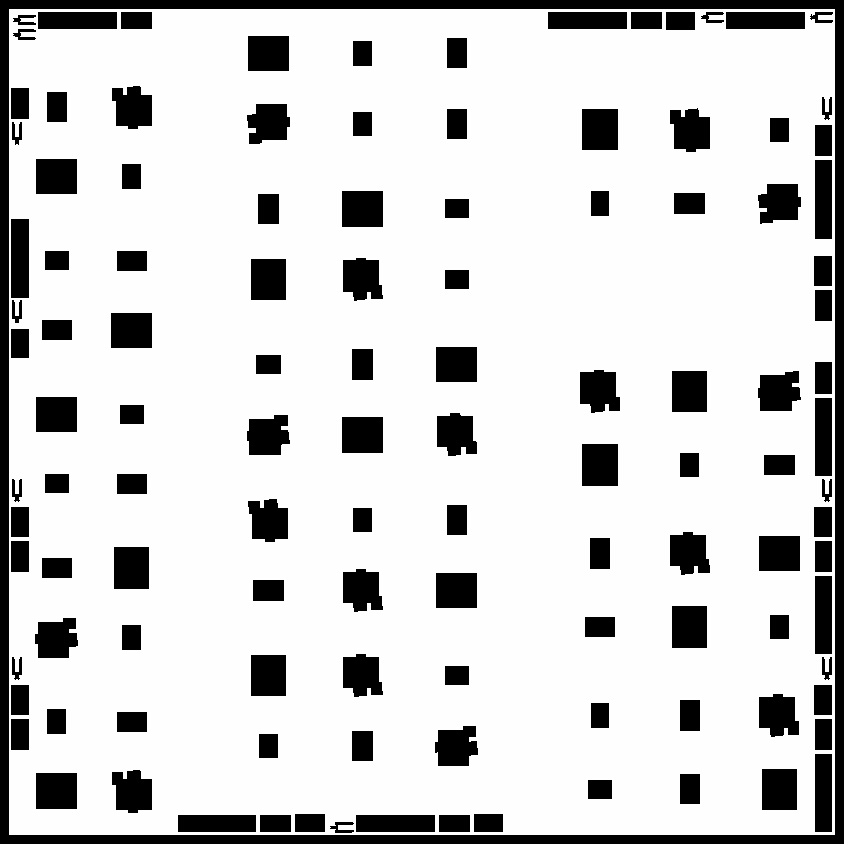
\includegraphics[width=\textwidth]{figures/warehouse_static_01.png}\\[0.4ex]
    {\footnotesize (a) static \texttt{\_01}, distributed}
  \end{minipage}\hfill
  \begin{minipage}[t]{0.32\textwidth}
    \centering
    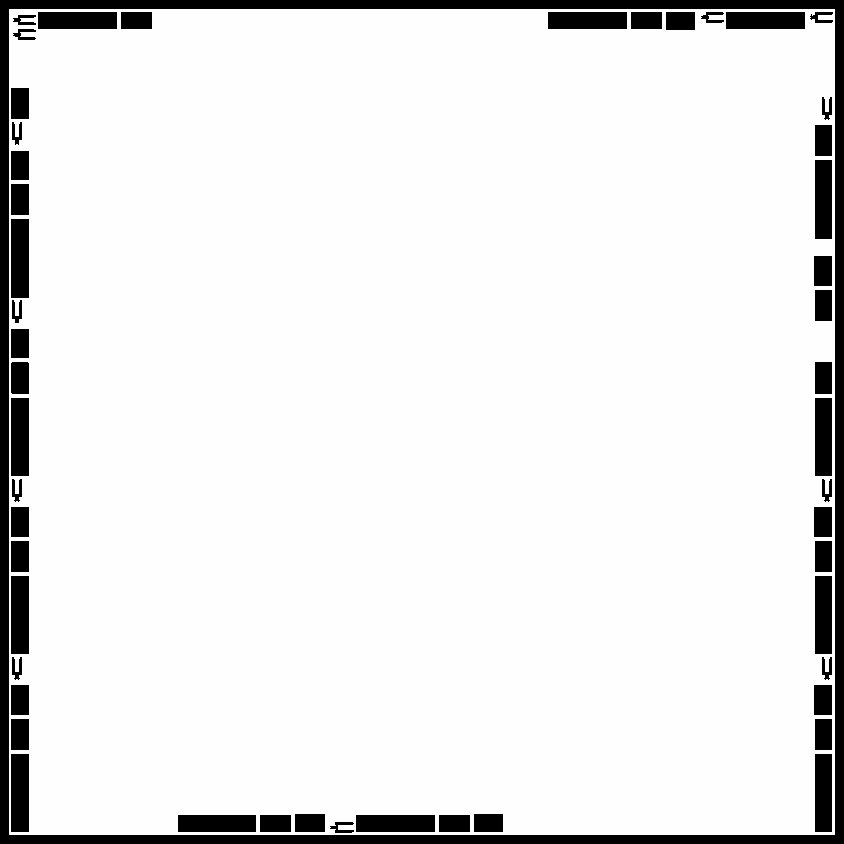
\includegraphics[width=\textwidth]{figures/warehouse_objonwallonly.png}\\[0.4ex]
    {\footnotesize (b) \texttt{objonwallonly}}
  \end{minipage}\hfill
  \begin{minipage}[t]{0.32\textwidth}
    \centering
    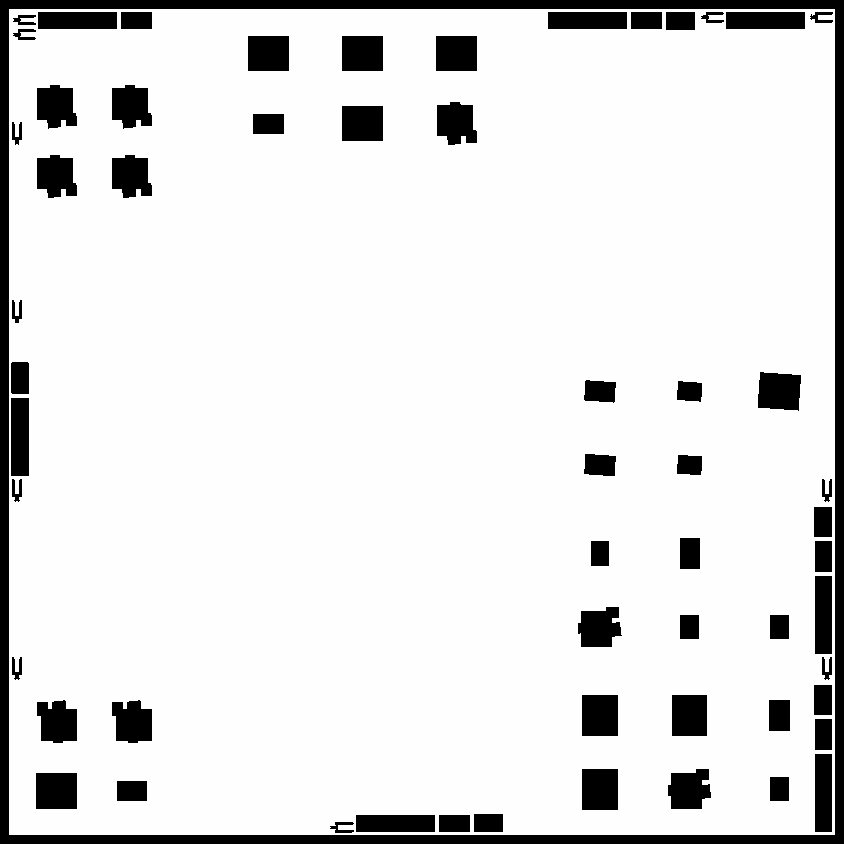
\includegraphics[width=\textwidth]{figures/warehouse_dynamic.png}\\[0.4ex]
    {\footnotesize (c) dynamic}
  \end{minipage}
  \caption[Baked occupancy truth of the three large-warehouse object arrangements, each \SI{42.2}{\metre} square at \SI{0.05}{\metre} per cell with origin $(-21.1,-21.1)$~m.]{Baked occupancy truth of the three large-warehouse object arrangements,
  each \SI{42.2}{\metre} square at \SI{0.05}{\metre} per cell with origin
  $(-21.1,-21.1)$~m. Black is occupied, white is free; there is no unknown space
  because the grids are rasterised from collision geometry rather than observed.
  Occupied cells are \SI{17.79}{\percent} of~(a), \SI{8.74}{\percent} of~(b) and
  \SI{10.98}{\percent} of~(c). Panel~(b) clears the central floor and keeps
  obstacles against the walls, which is the arrangement used by
  \repo{dataset_allsensor_002} and \repo{dataset_allsensor_003}. \emph{No
  occupancy grid is shown per floor treatment, and none exists:} the
  \texttt{bayline} and plain floors differ only in surface material, which carries
  no collision geometry, so their baked grids are identical to the panels above.
  See \cref{fig:floor-treatments}.}
  \label{fig:warehouse-maps}
\end{figure}

The floor treatment is a separate factor and is invisible to occupancy. It is set
by which ground model a world includes; those models share one mesh and differ only
in the visual materials attached to it (\cref{tab:floor-variants}).
\Cref{fig:floor-treatments} renders both recorded conditions at true scale using
\repo{script/render_floor.py}, which drives the 2-D viewer's own floor rasteriser
so that the figure shows what the overlay and the simulated cameras see rather
than a texture file out of context.

\begin{figure}[htbp]
  \centering
  \begin{minipage}[t]{0.33\textwidth}
    \centering
    
\includegraphics[width=\textwidth]{figures/floor_plain.png}\\[0.4ex]
    {\footnotesize (a) plain, \repo{allsensor_000}--\repo{_002}}
  \end{minipage}\hfill
  \begin{minipage}[t]{0.33\textwidth}
    \centering
    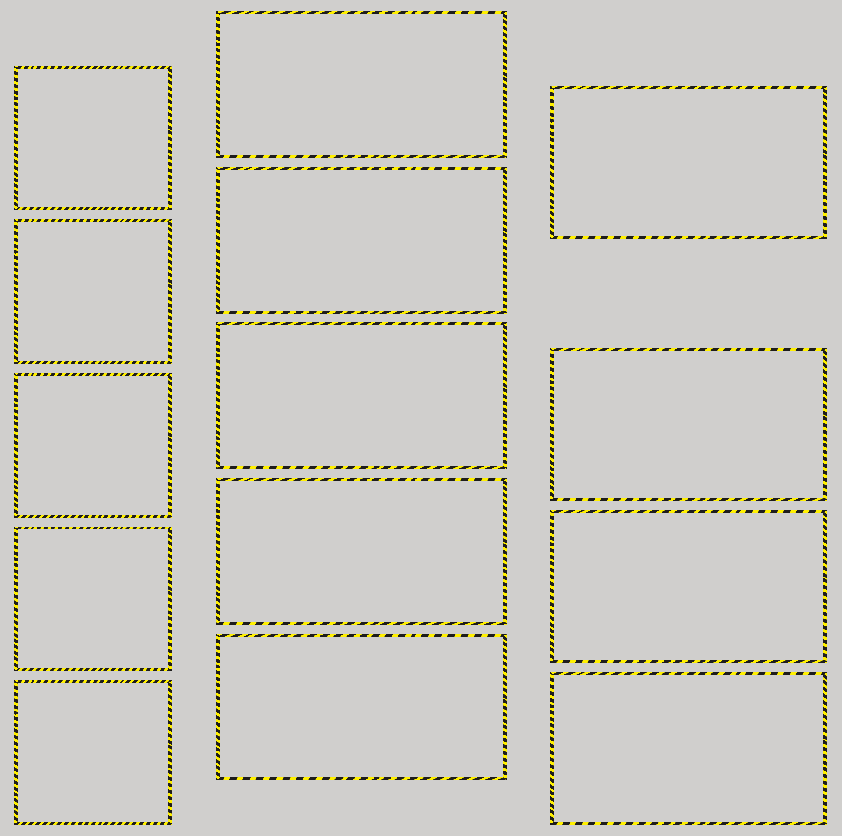
\includegraphics[width=\textwidth]{figures/floor_bayline.png}\\[0.4ex]
    {\footnotesize (b) \texttt{bayline}, \repo{allsensor_003}, \repo{_004}}
  \end{minipage}\hfill
  \begin{minipage}[t]{0.29\textwidth}
    \centering
    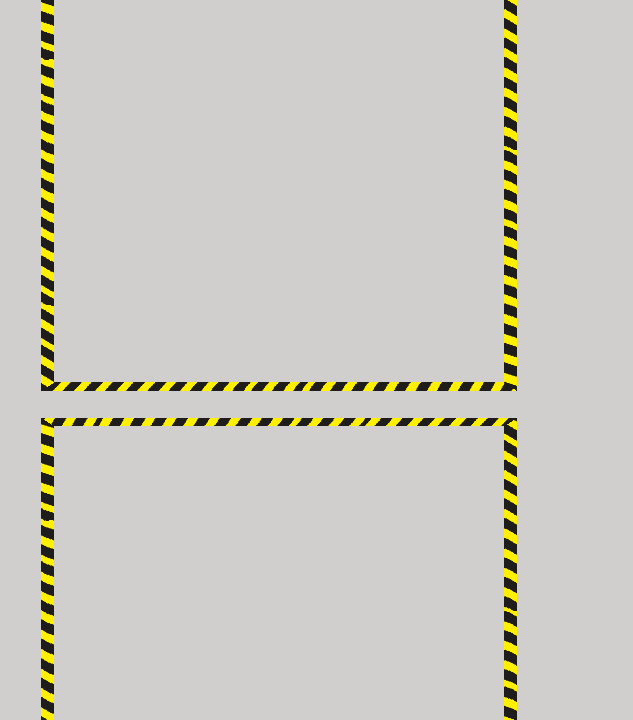
\includegraphics[width=\textwidth]{figures/floor_bayline_detail.png}\\[0.4ex]
    {\footnotesize (c) \SI{12}{\metre} detail of~(b)}
  \end{minipage}
  \caption[The two recorded floor conditions, rendered across the full \SI{42.2}{\metre} floor at \SI{0.05}{\metre} per pixel.]{The two recorded floor conditions, rendered across the full
  \SI{42.2}{\metre} floor at \SI{0.05}{\metre} per pixel. Both share the same flat
  diffuse base, RGB $(0.814,0.811,0.804)$; the only difference between them is the
  112 painted marking faces that \texttt{bayline} adds, forming the hazard-striped
  outlines of fourteen storage bays. Panel~(c) is a \SI{12}{\metre} square detail
  showing the strips at \SI{0.145}{\metre} width. Everything not outlined is
  untextured in both conditions.}
  \label{fig:floor-treatments}
\end{figure}

\begin{table}[htbp]
\centering
\caption[Ground models and the floor conditions they produce.]{Ground models and the floor conditions they produce. The mesh and its
collision geometry are identical in all three, so the floor treatment changes what
a camera sees and nothing a wheel, an occupancy grid or a collision check responds
to. The concrete-grain texture belongs to the stock model only, and no recorded
dataset uses it.}
\label{tab:floor-variants}
\small
\begin{tabularx}{\textwidth}{>{\raggedright\arraybackslash}p{0.29\textwidth}lll>{\raggedright\arraybackslash}X}
\toprule
Ground model & Base & Concrete & Markings & Used by \\
\midrule
\repo{..._GroundB_01} (stock) & texture & yes & 112 faces & no recorded dataset \\
\repo{..._GroundB_01_bayline} & flat diffuse & no & 112 faces &
  \repo{allsensor_003}, \repo{allsensor_004} \\
\repo{..._GroundB_01_plain} & flat diffuse & no & none &
  \repo{allsensor_000}--\repo{_002}, all \texttt{nofloortexture} datasets \\
\bottomrule
\end{tabularx}
\end{table}

\begin{queried}[Naming]
The factor recorded in this project as ``textured versus featureless floor'' is
narrower than the name suggests, and \cref{fig:floor-treatments} is the evidence.
Both conditions rest on the \emph{same flat, untextured diffuse colour}; the stock
concrete-grain texture appears in neither. The entire difference is fourteen
painted bay outlines, \SI{0.145}{\metre} wide, covering a small fraction of a
\SI{1704}{\metre\squared} floor. A robot driving an aisle sees a uniform grey
surface in both conditions for most of its path, crossing a high-contrast strip
only at a bay boundary.

Results comparing the two floors must therefore be read as \emph{bay markings
versus nothing}, not as \emph{realistic floor versus nothing}, and the near-absence
of a visual-odometry improvement between them (\cref{sec:results-proprio}) should
not be generalised to floors carrying genuine surface texture. Testing that would
require a world built on the stock \repo{GroundB_01} model, which no recorded
dataset uses.
\end{queried}

\begin{queried}[Unverified]
The dynamic world's baked grid, \cref{fig:warehouse-maps}(c), contains
\SI{38}{\percent} fewer occupied cells than the distributed static arrangement
in~(a). \repo{bake_map.py} rasterises every \texttt{<include>} in the
world file at its authored pose, so kinematically driven props should appear at
their initial positions, but this has not been confirmed for the dynamic family.
Until it is, panel~(c) must not be used as occupancy truth for scoring a
reconstructed map of a dynamic scene: the deficit may be a genuine difference in
static stocking, or it may be props missing from the bake, and those two
possibilities imply opposite corrections. The estimator results in
\cref{sec:results-proprio} are unaffected, as they use the arrangements in
panels~(a) and~(b) only.
\end{queried}

Each recorded dataset is the combination of three things that vary independently
and are easy to confuse when read off three separate artifacts: the floor
treatment, the object arrangement, and the route the robot actually drove.
\Cref{fig:dataset-scenes} draws all three together for every dataset, and
\cref{tab:dataset-scenes} gives the numbers behind the pictures. Both are produced
by \repo{script/render_dataset_scene.py}, which resolves each dataset's world from
its own run manifest rather than from its name---necessary because
\repo{dataset_static_nofloortexture_001} sits in the \texttt{\_01} arrangement
while \repo{_000} and \repo{_002} sit in the canonical one, and all three carry
\texttt{nofloortexture} in the name.

\begin{figure}[p]
  \centering
  \begin{minipage}[t]{0.235\textwidth}
    \centering
    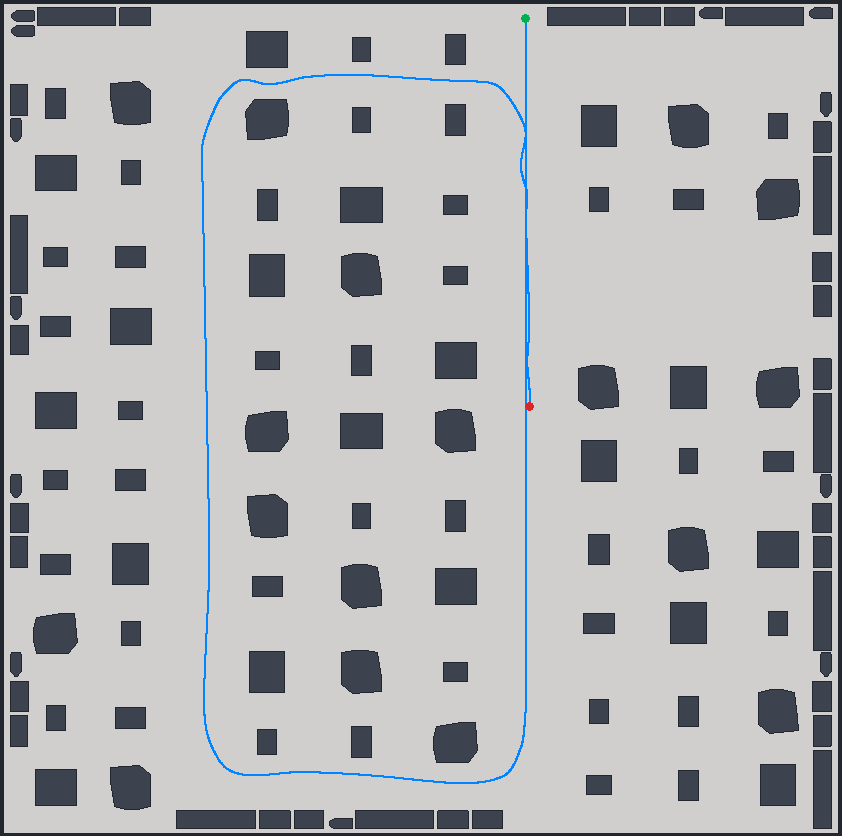
\includegraphics[width=\textwidth]{figures/scene_allsensor_000.png}\\[0.3ex]
    {\scriptsize \repo{allsensor_000}}
  \end{minipage}\hfill
  \begin{minipage}[t]{0.235\textwidth}
    \centering
    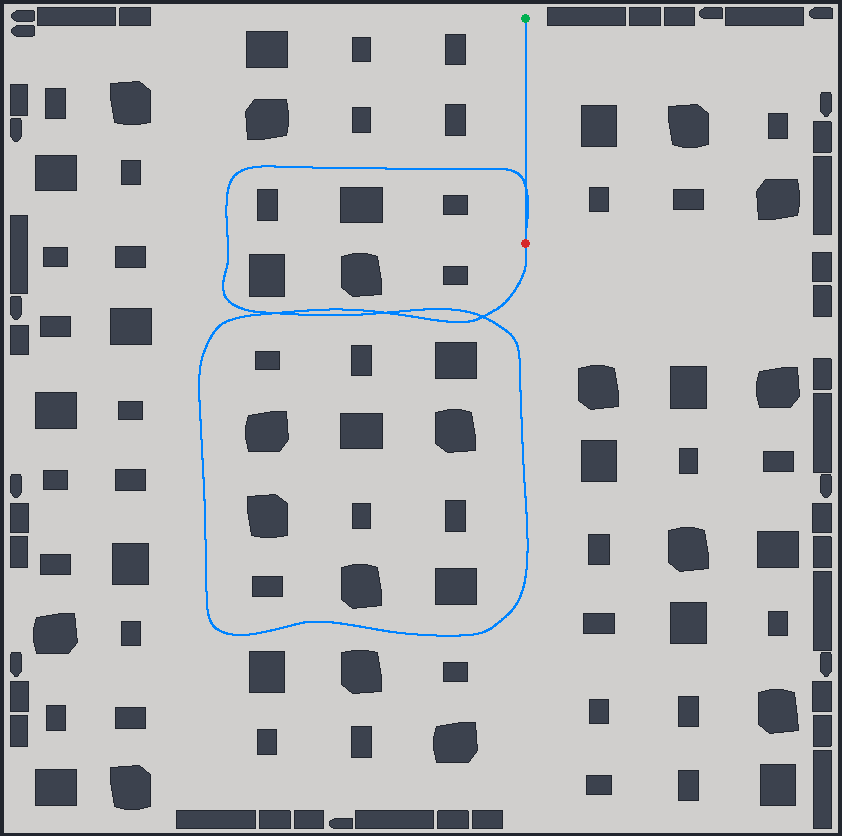
\includegraphics[width=\textwidth]{figures/scene_allsensor_001.png}\\[0.3ex]
    {\scriptsize \repo{allsensor_001}}
  \end{minipage}\hfill
  \begin{minipage}[t]{0.235\textwidth}
    \centering
    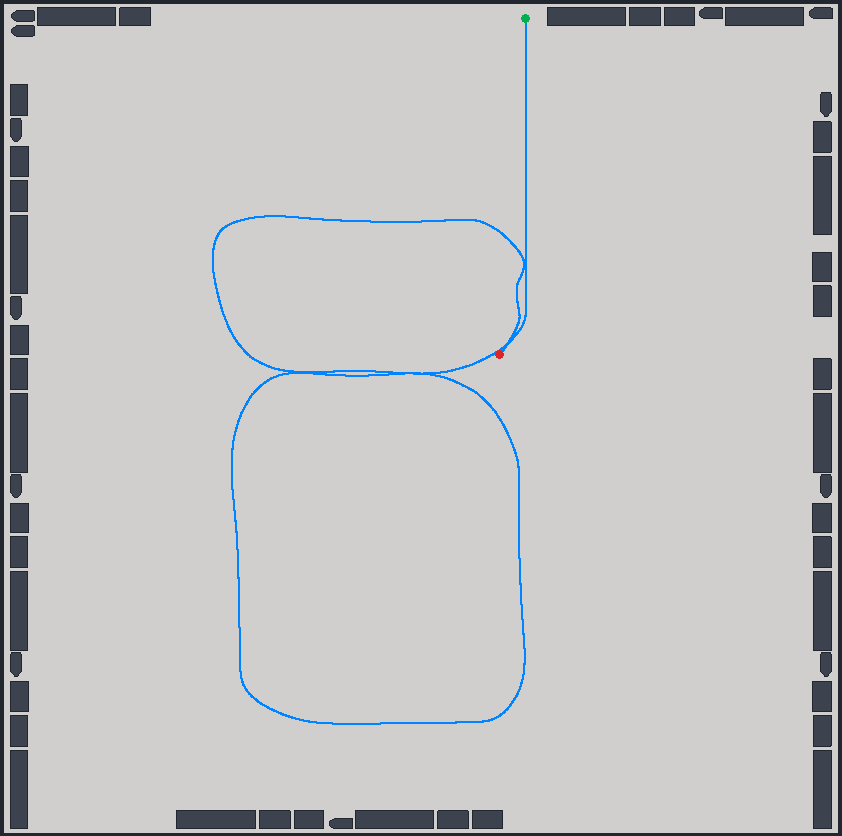
\includegraphics[width=\textwidth]{figures/scene_allsensor_002.png}\\[0.3ex]
    {\scriptsize \repo{allsensor_002}}
  \end{minipage}\hfill
  \begin{minipage}[t]{0.235\textwidth}
    \centering
    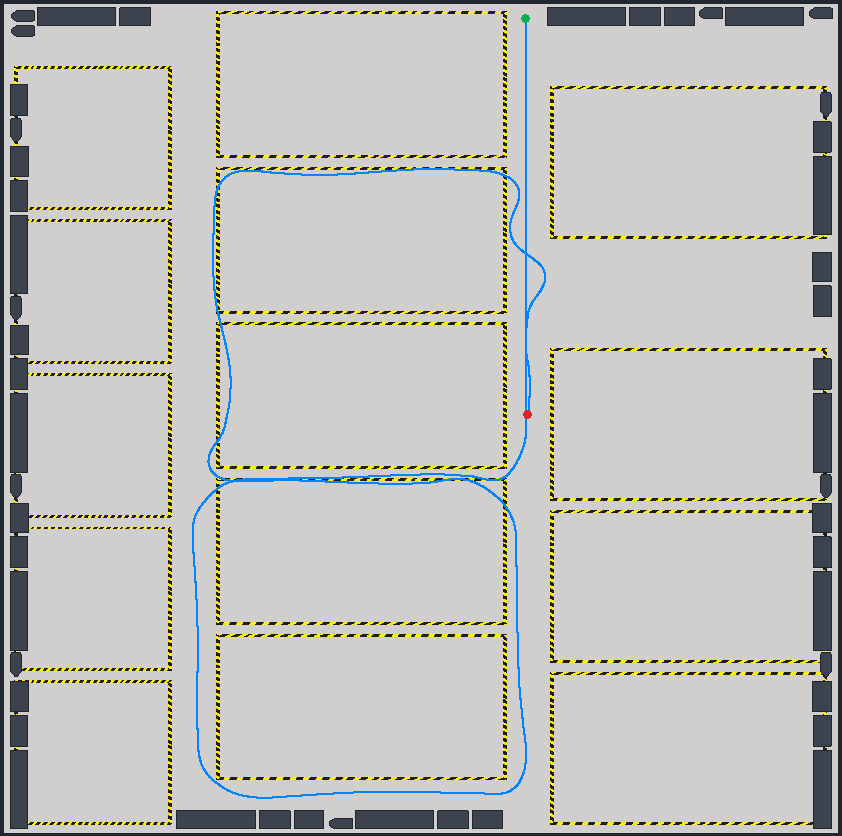
\includegraphics[width=\textwidth]{figures/scene_allsensor_003.png}\\[0.3ex]
    {\scriptsize \repo{allsensor_003}}
  \end{minipage}

  \vspace{1.2ex}
  \begin{minipage}[t]{0.235\textwidth}
    \centering
    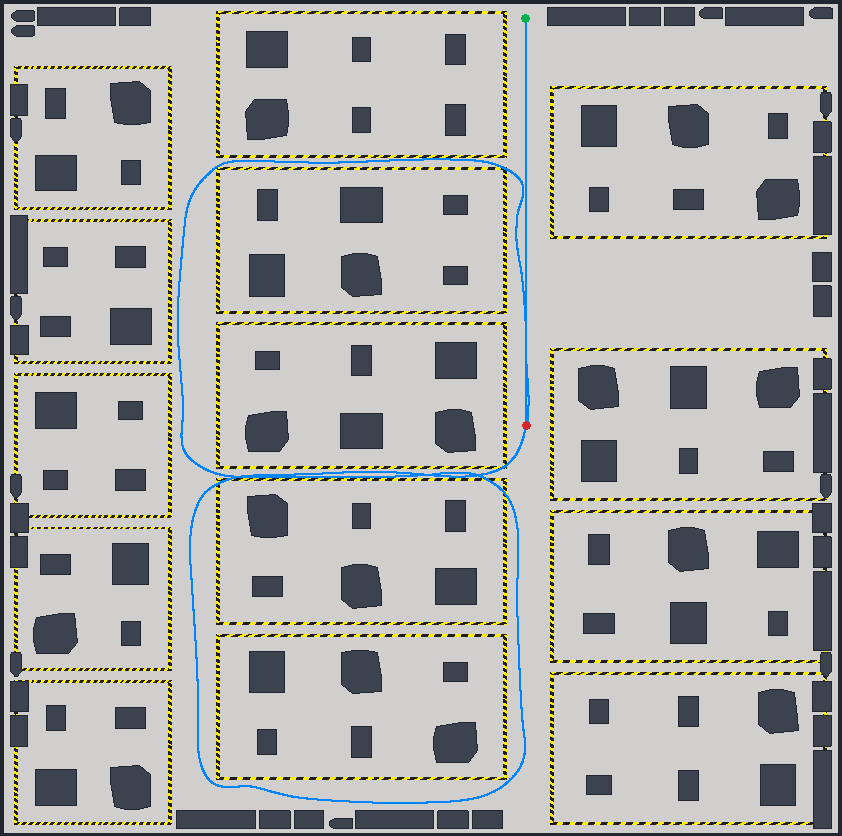
\includegraphics[width=\textwidth]{figures/scene_allsensor_004.png}\\[0.3ex]
    {\scriptsize \repo{allsensor_004}}
  \end{minipage}\hfill
  \begin{minipage}[t]{0.235\textwidth}
    \centering
    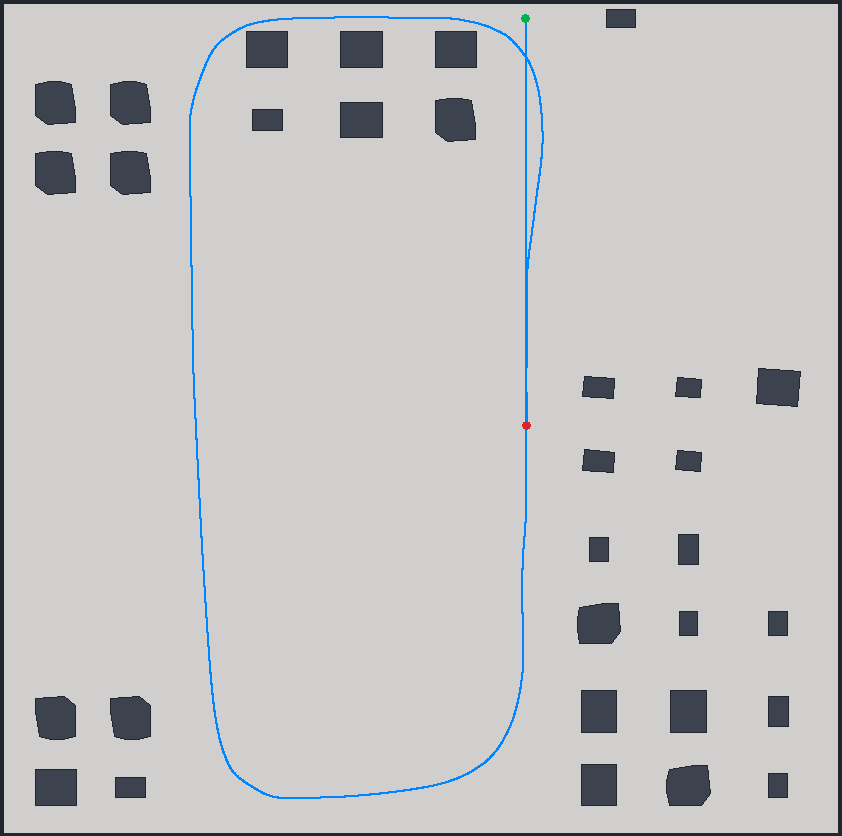
\includegraphics[width=\textwidth]{figures/scene_static_nofloortexture_000.png}\\[0.3ex]
    {\scriptsize \repo{static_000}\flag{*}}
  \end{minipage}\hfill
  \begin{minipage}[t]{0.235\textwidth}
    \centering
    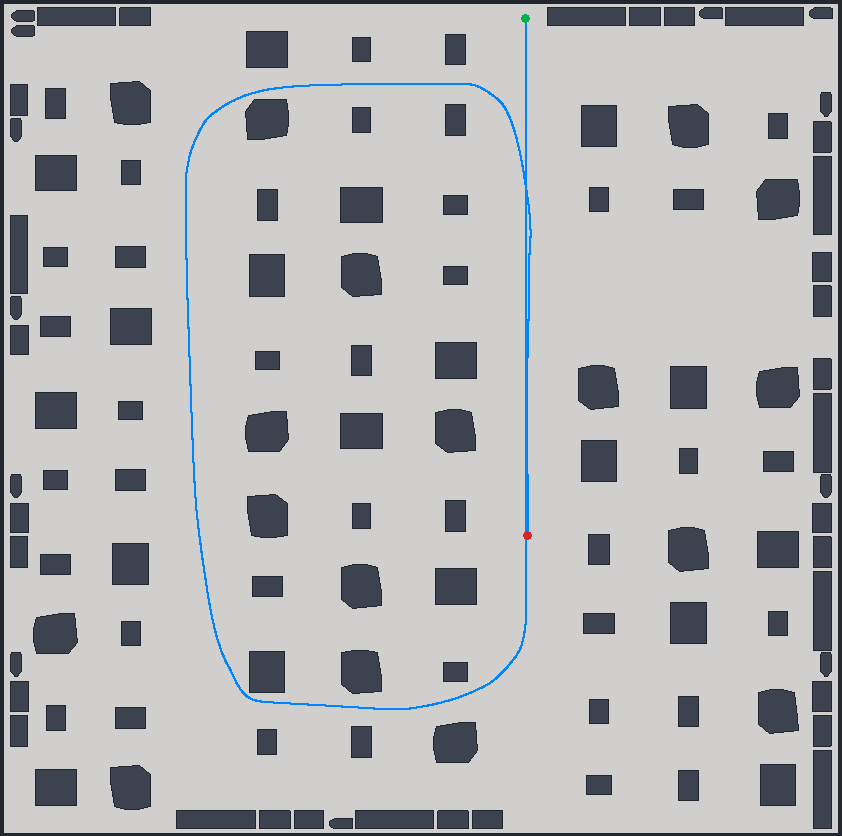
\includegraphics[width=\textwidth]{figures/scene_static_nofloortexture_001.png}\\[0.3ex]
    {\scriptsize \repo{static_001}}
  \end{minipage}\hfill
  \begin{minipage}[t]{0.235\textwidth}
    \centering
    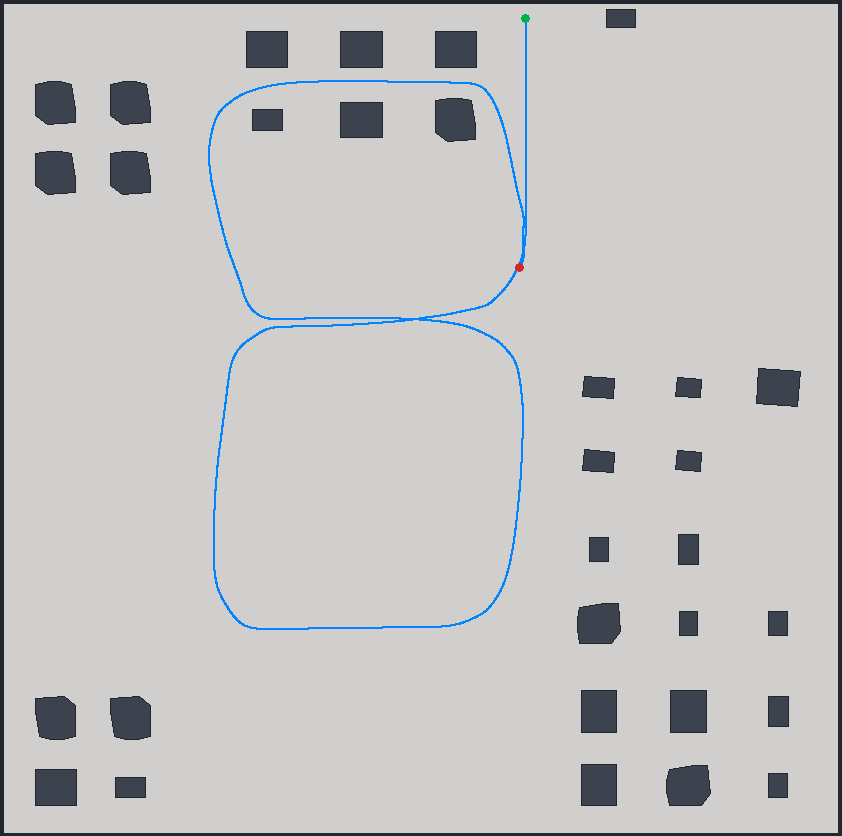
\includegraphics[width=\textwidth]{figures/scene_static_nofloortexture_002.png}\\[0.3ex]
    {\scriptsize \repo{static_002}\flag{*}}
  \end{minipage}

  \vspace{1.2ex}
  \begin{minipage}[t]{0.235\textwidth}
    \centering
    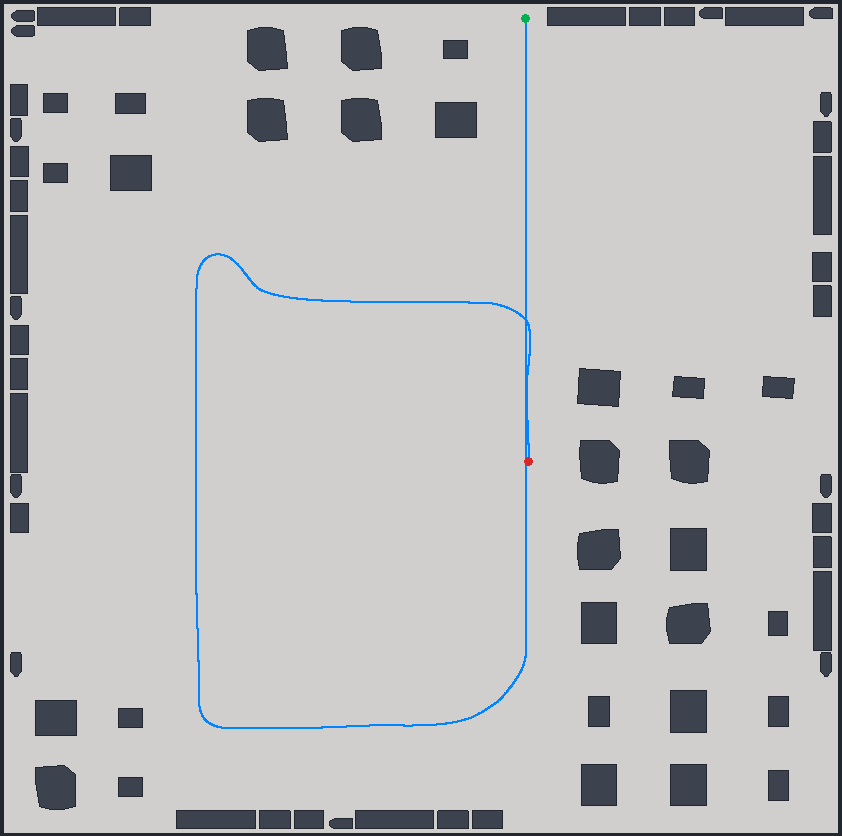
\includegraphics[width=\textwidth]{figures/scene_dynamic_nofloortexture_00_000.png}\\[0.3ex]
    {\scriptsize \repo{dynamic_00_000}}
  \end{minipage}\hfill
  \begin{minipage}[t]{0.235\textwidth}
    \centering
    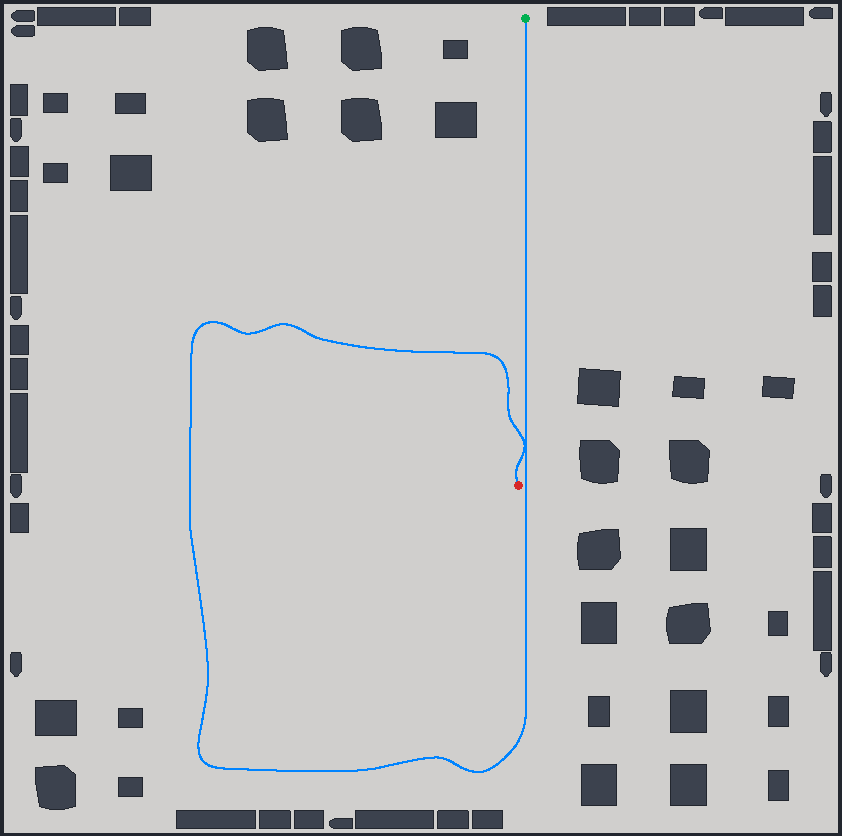
\includegraphics[width=\textwidth]{figures/scene_dynamic_nofloortexture_00_001.png}\\[0.3ex]
    {\scriptsize \repo{dynamic_00_001}}
  \end{minipage}\hfill
  \begin{minipage}[t]{0.235\textwidth}
    \centering
    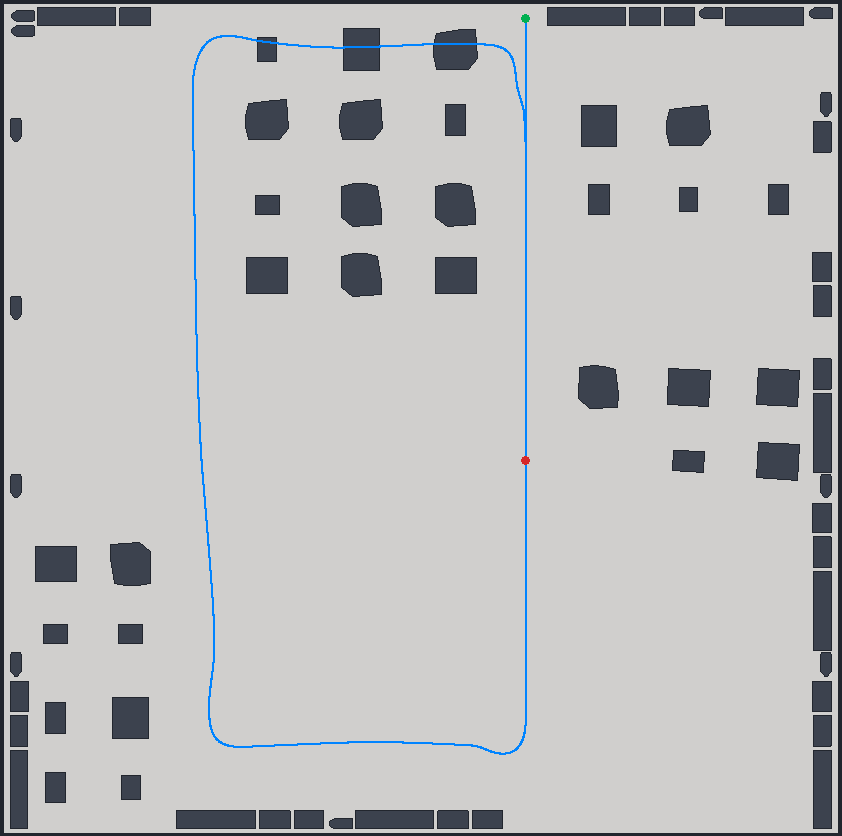
\includegraphics[width=\textwidth]{figures/scene_dynamic_nofloortexture_01_000.png}\\[0.3ex]
    {\scriptsize \repo{dynamic_01_000}}
  \end{minipage}\hfill
  \begin{minipage}[t]{0.235\textwidth}
    \centering
    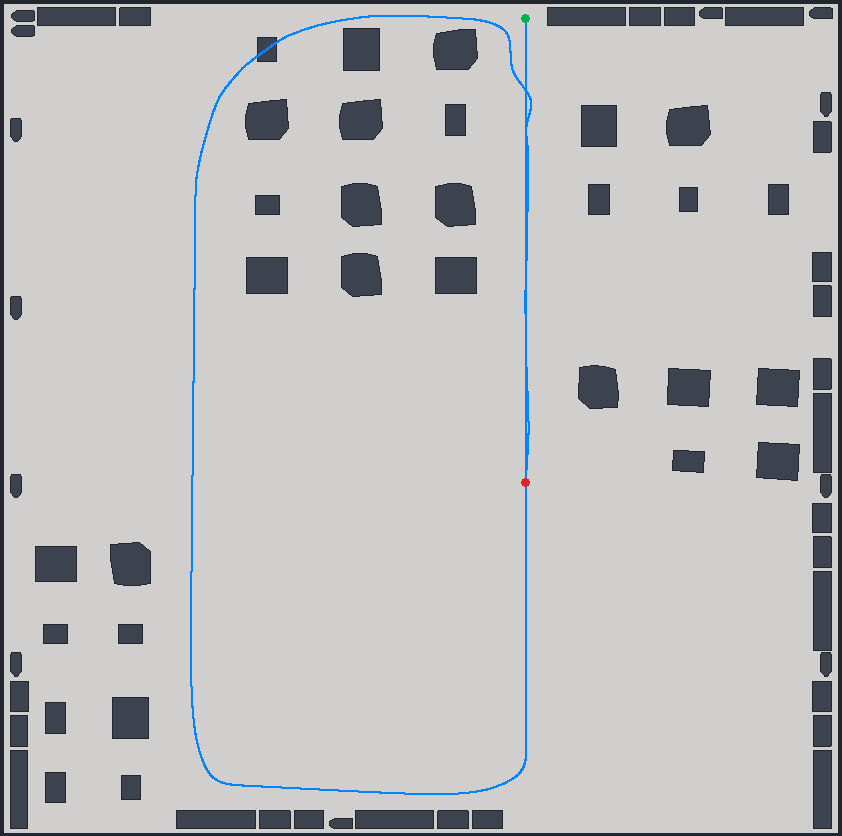
\includegraphics[width=\textwidth]{figures/scene_dynamic_nofloortexture_02_000.png}\\[0.3ex]
    {\scriptsize \repo{dynamic_02_000}}
  \end{minipage}
  \caption[Every simulation dataset as a scene: floor treatment, object layout and ground-truth route in one view.]{Every simulation dataset as a scene: floor treatment, object layout and
  ground-truth route in one view. Grey is open floor; dark polygons are obstacle
  footprints, taken as convex hulls of each collision mesh sliced at robot height,
  the same geometry the occupancy bake uses. Yellow hazard striping is the painted
  bay outline of the \texttt{bayline} floor and is absent on plain floors. The blue
  trace is the recorded \repo{/ground_truth/odometry} route, green marking its
  start and red its end. Moving props are drawn at their authored pose, which is
  where the world file places them at $t=0$; this is a layout figure and does not
  show where a prop was at any instant during a dynamic recording. \flag{*}~marks a
  dataset whose recorded world no longer exists and whose objects were
  reconstructed---see the note below \cref{tab:dataset-scenes}.}
  \label{fig:dataset-scenes}
\end{figure}

\begin{table}[htbp]
\centering
\caption[What each dataset contains.]{What each dataset contains. ``Objects'' counts obstacle instances whose
collision geometry intersects the robot-height band, excluding the wall ring.
``Route'' is the ground-truth path length and ``sim span'' its duration in
simulated time. The world column drops the floor suffix, which is given separately,
so two rows sharing a world arrangement but differing in floor are visible as such.}
\label{tab:dataset-scenes}
\footnotesize
\setlength{\tabcolsep}{3pt}
%% Generated by script/render_dataset_scene.py -- do not edit.
\begin{tabularx}{\textwidth}{>{\raggedright\arraybackslash}Xllrrrr}
\toprule
Dataset & World & Floor & Objects & Route & Sim span & Truth \\
 & arrangement & & & [\si{\metre}] & [\si{\second}] & samples \\
\midrule
\repo{dataset_allsensor_000} & \texttt{static\_01} & plain & 117 & 117.0 & 87.1 & 4354 \\
\repo{dataset_allsensor_001} & \texttt{static\_01} & plain & 117 & 113.1 & 81.8 & 4091 \\
\repo{dataset_allsensor_002} & \texttt{static\_objonwallonly} & plain & 49 & 115.2 & 86.7 & 4338 \\
\repo{dataset_allsensor_003} & \texttt{static\_objonwallonly} & bayline & 49 & 140.6 & 102.4 & 5119 \\
\repo{dataset_allsensor_004} & \texttt{static\_01} & bayline & 117 & 142.3 & 100.5 & 5026 \\
\repo{dataset_dynamic_nofloortexture_00_000} & \texttt{dynamic\_00} & plain & 69 & 97.1 & 77.4 & 3873 \\
\repo{dataset_dynamic_nofloortexture_00_001} & \texttt{dynamic\_00} & plain & 69 & 97.3 & 74.2 & 3710 \\
\repo{dataset_dynamic_nofloortexture_01_000} & \texttt{dynamic\_01} & plain & 68 & 122.8 & 84.6 & 4230 \\
\repo{dataset_dynamic_nofloortexture_02_000} & \texttt{dynamic\_02} & plain & 68 & 126.6 & 89.5 & 4475 \\
\repo{dataset_static_nofloortexture_000}\flag{*} & \texttt{static} & plain & 31 & 122.9 & 86.7 & 4334 \\
\repo{dataset_static_nofloortexture_001} & \texttt{static\_01} & plain & 117 & 113.1 & 82.0 & 4100 \\
\repo{dataset_static_nofloortexture_002}\flag{*} & \texttt{static} & plain & 31 & 114.7 & 89.5 & 4475 \\
\bottomrule
\end{tabularx}

\end{table}

\begin{queried}[Missing world]
\repo{dataset_static_nofloortexture_000} and \repo{_002} name
\repo{worlds/small_warehouse_static/small_warehouse_static_nofloortexture.world}
in their run manifests, and \flag{that file no longer exists in the repository}.
Both datasets contribute to the relogged campaign of \cref{sec:results-validity},
so their scenes could not be drawn from the recorded world and their conditions
cannot be re-inspected directly.

The panels marked \flag{*} are reconstructions. They are exact for geometry rather
than approximate, because \repo{script/make_plain_floor.py} produces a floor
variant by swapping only the ground model's \texttt{<include>} URI and leaves every
object untouched: the missing world therefore differed from the surviving
\repo{small_warehouse_static.world} in its floor alone, and that floor is
recoverable from the suffix. It remains a reconstruction and not the recorded file,
and the two datasets should be re-recorded, or the world restored from history,
before either is used for anything the floor or the object layout bears on.
\end{queried}

The available controlled factors are summarised in \cref{tab:controlled-factors}.

\begin{table}[htbp]
\centering
\caption[Controlled experimental factors available in the simulation environment, with the levels realised at the reporting cutoff.]{Controlled experimental factors available in the simulation environment,
with the levels realised at the reporting cutoff. A factor is listed as exercised
only where a recorded dataset exists for more than one of its levels.}
\label{tab:controlled-factors}
\small
\begin{tabularx}{\textwidth}{>{\raggedright\arraybackslash}p{0.21\textwidth}>{\raggedright\arraybackslash}p{0.30\textwidth}>{\raggedright\arraybackslash}X}
\toprule
Factor & Levels & Status at cutoff \\
\midrule
Scene dynamics & static props; scripted dynamic props & exercised \\
Floor markings & bay outlines present (\texttt{bayline});
  absent (plain) & exercised; no dataset carries surface texture \\
Prop or route arrangement & canonical; \texttt{\_00}; \texttt{\_01};
  \texttt{\_02} & exercised \\
Stocking level & partial; fully stocked static & fully stocked recorded \\
Object placement & distributed; restricted to the wall region & exercised, three
  bags to one \\
Domain & simulation; real robot & exercised, no real ground truth \\
World scale & tiny \repo{small_warehouse}; large rescaled families & distinct
  environments, never pooled \\
\bottomrule
\end{tabularx}
\end{table}

The plain floor removes the painted bay outlines; neither recorded condition
carries the stock concrete texture. Collision geometry and occupancy truth are
preserved in both (\cref{tab:floor-variants}). Dynamic props follow
deterministic routes through a kinematic Gazebo plugin. This preserves repeatable
motion and acceptable real-time factor, but it does not reproduce physical
collision response if the robot overlaps a moving prop.

World identity is recorded by exact \texttt{.world} path. ROS launches require
\repo{colcon build --symlink-install}; a plain build can leave an obsolete copied
world in \repo{install/}. When object motion is required by the 2-D viewer, model
poses must also be bridged from the simulator.
